
%%%%%%%%%%%%%%%%%%%%%%%%%%%%%%%%%%%%%%%%%%%%%%%%%%%%%%%%%%%%%%%%%%%%%%%%%%%%%%%%
%%%%%%%%%%% Document class and package options
%%%%%%%%%%%%%%%%%%%%%%%%%%%%%%%%%%%%%%%%%%%%%%%%%%%%%%%%%%%%%%%%%%%%%%%%%%%%%%%%
% \documentclass[a4paper,12pt]{article}
\documentclass[a4paper,12pt,twoside]{article}
\usepackage{outline}

\usepackage{amsmath}
\usepackage{amssymb}                    % AMS Math
\usepackage{amsfonts}
\usepackage[tight,hang,centerlast]{subfigure}
\usepackage[lined,ruled,longend]{algorithm2e}
\usepackage{longtable}
\usepackage{verbatim}

%\usepackage[dvipsnames]{xcolor}

\usepackage{rotating}

\usepackage{fancyvrb}




\clubpenalty=1000
\widowpenalty=1000

%% eps to pdf
%% specify .eps extension when \includegraphics if you want the .pdf fig file to
%%     be regenerated as part of the compilation. Without extension the .pdf fig
%%     file is generated only if it does not exist yet
%% --shell-escape option must be enabled
\newif\ifpdf
\ifx\pdfoutput\undefined
   \pdffalse
\else
   \pdfoutput=1
   \pdftrue
\fi
\ifpdf
   \usepackage{graphicx}
   \usepackage{epstopdf}

   \epstopdfsetup{suffix=}

   \DeclareGraphicsRule{.eps}{pdf}{.pdf}{`epstopdf #1}
   \pdfcompresslevel=9
\else
   \usepackage{graphicx}
\fi


\begin{document}


%%%%%%%%%%%%%%%%%%%%%%%%%%%%%%%%%%%%%%%%%%%%%%%%%%%%%%%%%%%%%%%%%%%%%%%%%%%%%%%%
%%%%%%%%%%% Title
%%%%%%%%%%%%%%%%%%%%%%%%%%%%%%%%%%%%%%%%%%%%%%%%%%%%%%%%%%%%%%%%%%%%%%%%%%%%%%%%

\title{Measurement Results from\\
Wireless Battle Mesh\\
Version 6}


%\date{April, 2013}

\contributors{WBM community}
\eventlocation{Aalborg University. Aalborg, Denmark}
\eventdates{15th to 21st of April 2013}
\eventurl{http://battlemesh.org/BattleMeshV6}
\doctype{Measurement Analysis (work in progress)}
\logofigure{figures/battlemeshv6}

\frontmatter

\maketitle

%%%%%%%%%%%%%%%%%%%%%%%%%%%%%%%%%%%%%%%%%%%%%%%%%%%%%%%%%%%%%%%%%%%%%%%%%%%%%%%%
%%%%%%%%%%% Indices
%%%%%%%%%%%%%%%%%%%%%%%%%%%%%%%%%%%%%%%%%%%%%%%%%%%%%%%%%%%%%%%%%%%%%%%%%%%%%%%%

\thispagestyle{plain}
%\vspace*{3cm}

%\begin{center}
%\LARGE{\textbf{Abstract}} 
%\end{center}

%\begin{itemize}
%\item TODO..
%\end{itemize}

%\cleardoublepage
\clearsinglepage

\thispagestyle{plain}
\tableofcontents

%\cleardoublepage
\clearsinglepage

%%%%%%%%%%%%%%%%%%%%%%%%%%%%%%%%%%%%%%%%%%%%%%%%%%%%%%%%%%%%%%%%%%%%%%%%%%%%%%%%
%%%%%%%%%%% The document
%%%%%%%%%%%%%%%%%%%%%%%%%%%%%%%%%%%%%%%%%%%%%%%%%%%%%%%%%%%%%%%%%%%%%%%%%%%%%%%%

\singlespacing
\mainmatter
%%%%%%%%%%%%%%%%%%%%%%%%%%%%%%%%%%%%%%%%%%%%%%%%%%%%%%%%%%%%%%%%%%%%%%%%%%%%%%%%
%%%%%%%%%%% Chapter Inclusion
%%%%%%%%%%%%%%%%%%%%%%%%%%%%%%%%%%%%%%%%%%%%%%%%%%%%%%%%%%%%%%%%%%%%%%%%%%%%%%%%


%%%%%%%%%%%%%%%%%%%%%%%%%%%%%%%%%%%%%%%%%%%%%%%%%%%%%%%%%%%%%%%%%%%%%%%%%%%%%%%%
%%%%%%%%%%%%%%%%%%%%%%%%%%%%%%%%%%%%%%%%%%%%%%%%%%%%%%%%%%%%%%%%%%%%%%%%%%%%%%%%
\thispagestyle{plain}

%%%%%%%%%%%%%%%%%%%%%%%%%%%%%%%%%%%%%%%%%%%%%%%%%%%%%%%%%%%%%%%%%%%%%%%%%%%%%%%%
%%%%%%%%%%%%%%%%%%%%%%%%%%%%%%%%%%%%%%%%%%%%%%%%%%%%%%%%%%%%%%%%%%%%%%%%%%%%%%%%
%%%%%%%%%%%%%%%%%%%%%%%%%%%%%%%%%%%%%%%%%%%%%%%%%%%%%%%%%%%%%%%%%%%%%%%%%%%%%%%%
\section{Introduction}
\label{sec:introduction}


WBM...

%%%%%%%%%%%%%%%%%%%%%%%%%%%%%%%%%%%%%%%%%%%%%%%%%%%%%%%%%%%%%%%%%%%%%%%%%%%%%%%%
%%%%%%%%%%%%%%%%%%%%%%%%%%%%%%%%%%%%%%%%%%%%%%%%%%%%%%%%%%%%%%%%%%%%%%%%%%%%%%%%
%%%%%%%%%%%%%%%%%%%%%%%%%%%%%%%%%%%%%%%%%%%%%%%%%%%%%%%%%%%%%%%%%%%%%%%%%%%%%%%%
% A summary of protocol itself, the used versions and configuration

%\section{Protocols}


%\subsection{Babel}

%\subsection{Batman-adv}

%\subsection{Bmx6}

%\subsection{OLSR}


%%%%%%%%%%%%%%%%%%%%%%%%%%%%%%%%%%%%%%%%%%%%%%%%%%%%%%%%%%%%%%%%%%%%%%%%%%%%%%%%
%%%%%%%%%%%%%%%%%%%%%%%%%%%%%%%%%%%%%%%%%%%%%%%%%%%%%%%%%%%%%%%%%%%%%%%%%%%%%%%%
%%%%%%%%%%%%%%%%%%%%%%%%%%%%%%%%%%%%%%%%%%%%%%%%%%%%%%%%%%%%%%%%%%%%%%%%%%%%%%%%
\section{Testbed Descripiton}

\subsection{Node System}

\subsection{Topology}

% wget http://downloads.battlemesh.org/WBMv6/geographical_map1.png
% wget http://downloads.battlemesh.org/WBMv6/geographical_map2.png
\begin{figure}[!ht]
\centering
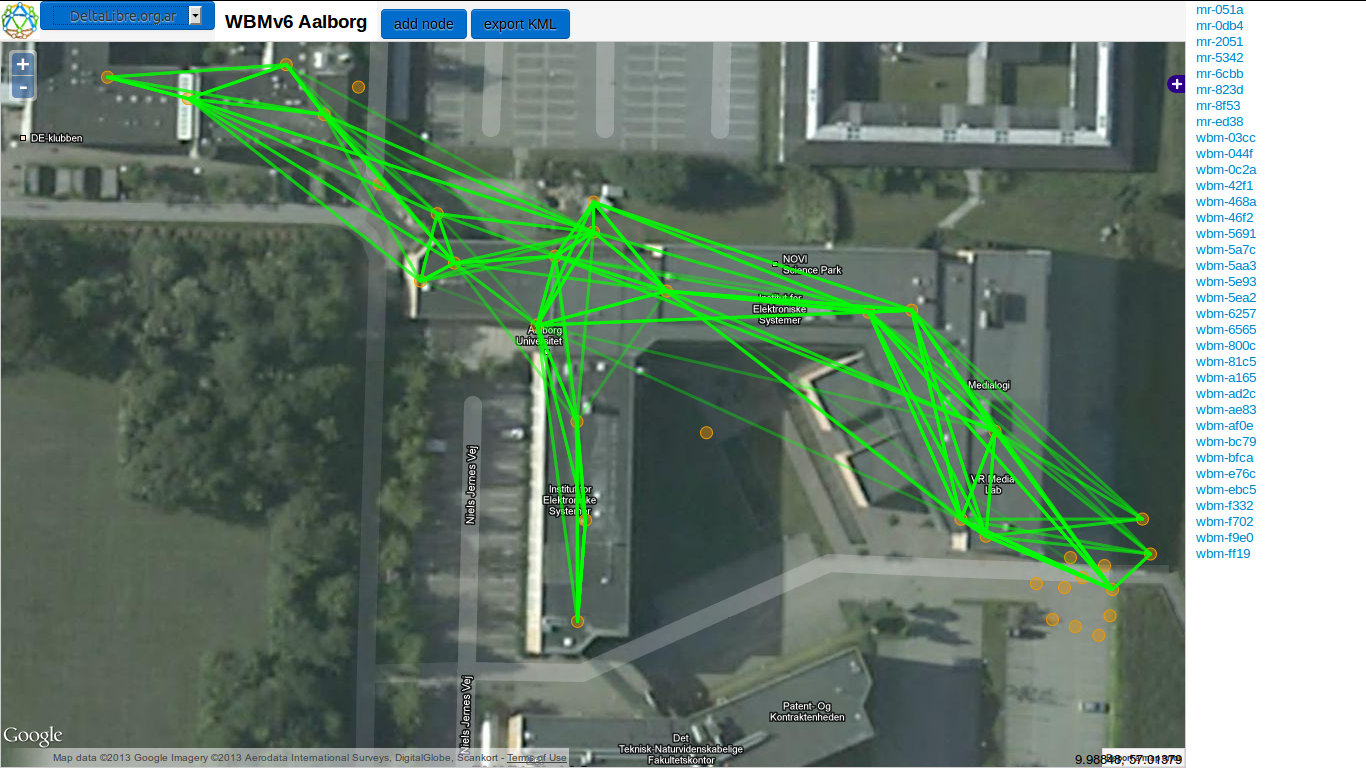
\includegraphics[width=1.4\textwidth, angle=90]{figures/geographical_map2.png}
\caption{geographical map snapshot}
\label{fig:geomap}
\end{figure}


% wget -O topo0.svg "http://battlemesh.org/BattleMeshV6/Tests?action=AttachFile&do=get&target=topo0.svg"
% \immediate\write18{ inkscape -D -z --file=topo0.svg --export-pdf=topo0.pdf }

\begin{figure}[!ht]
\centering
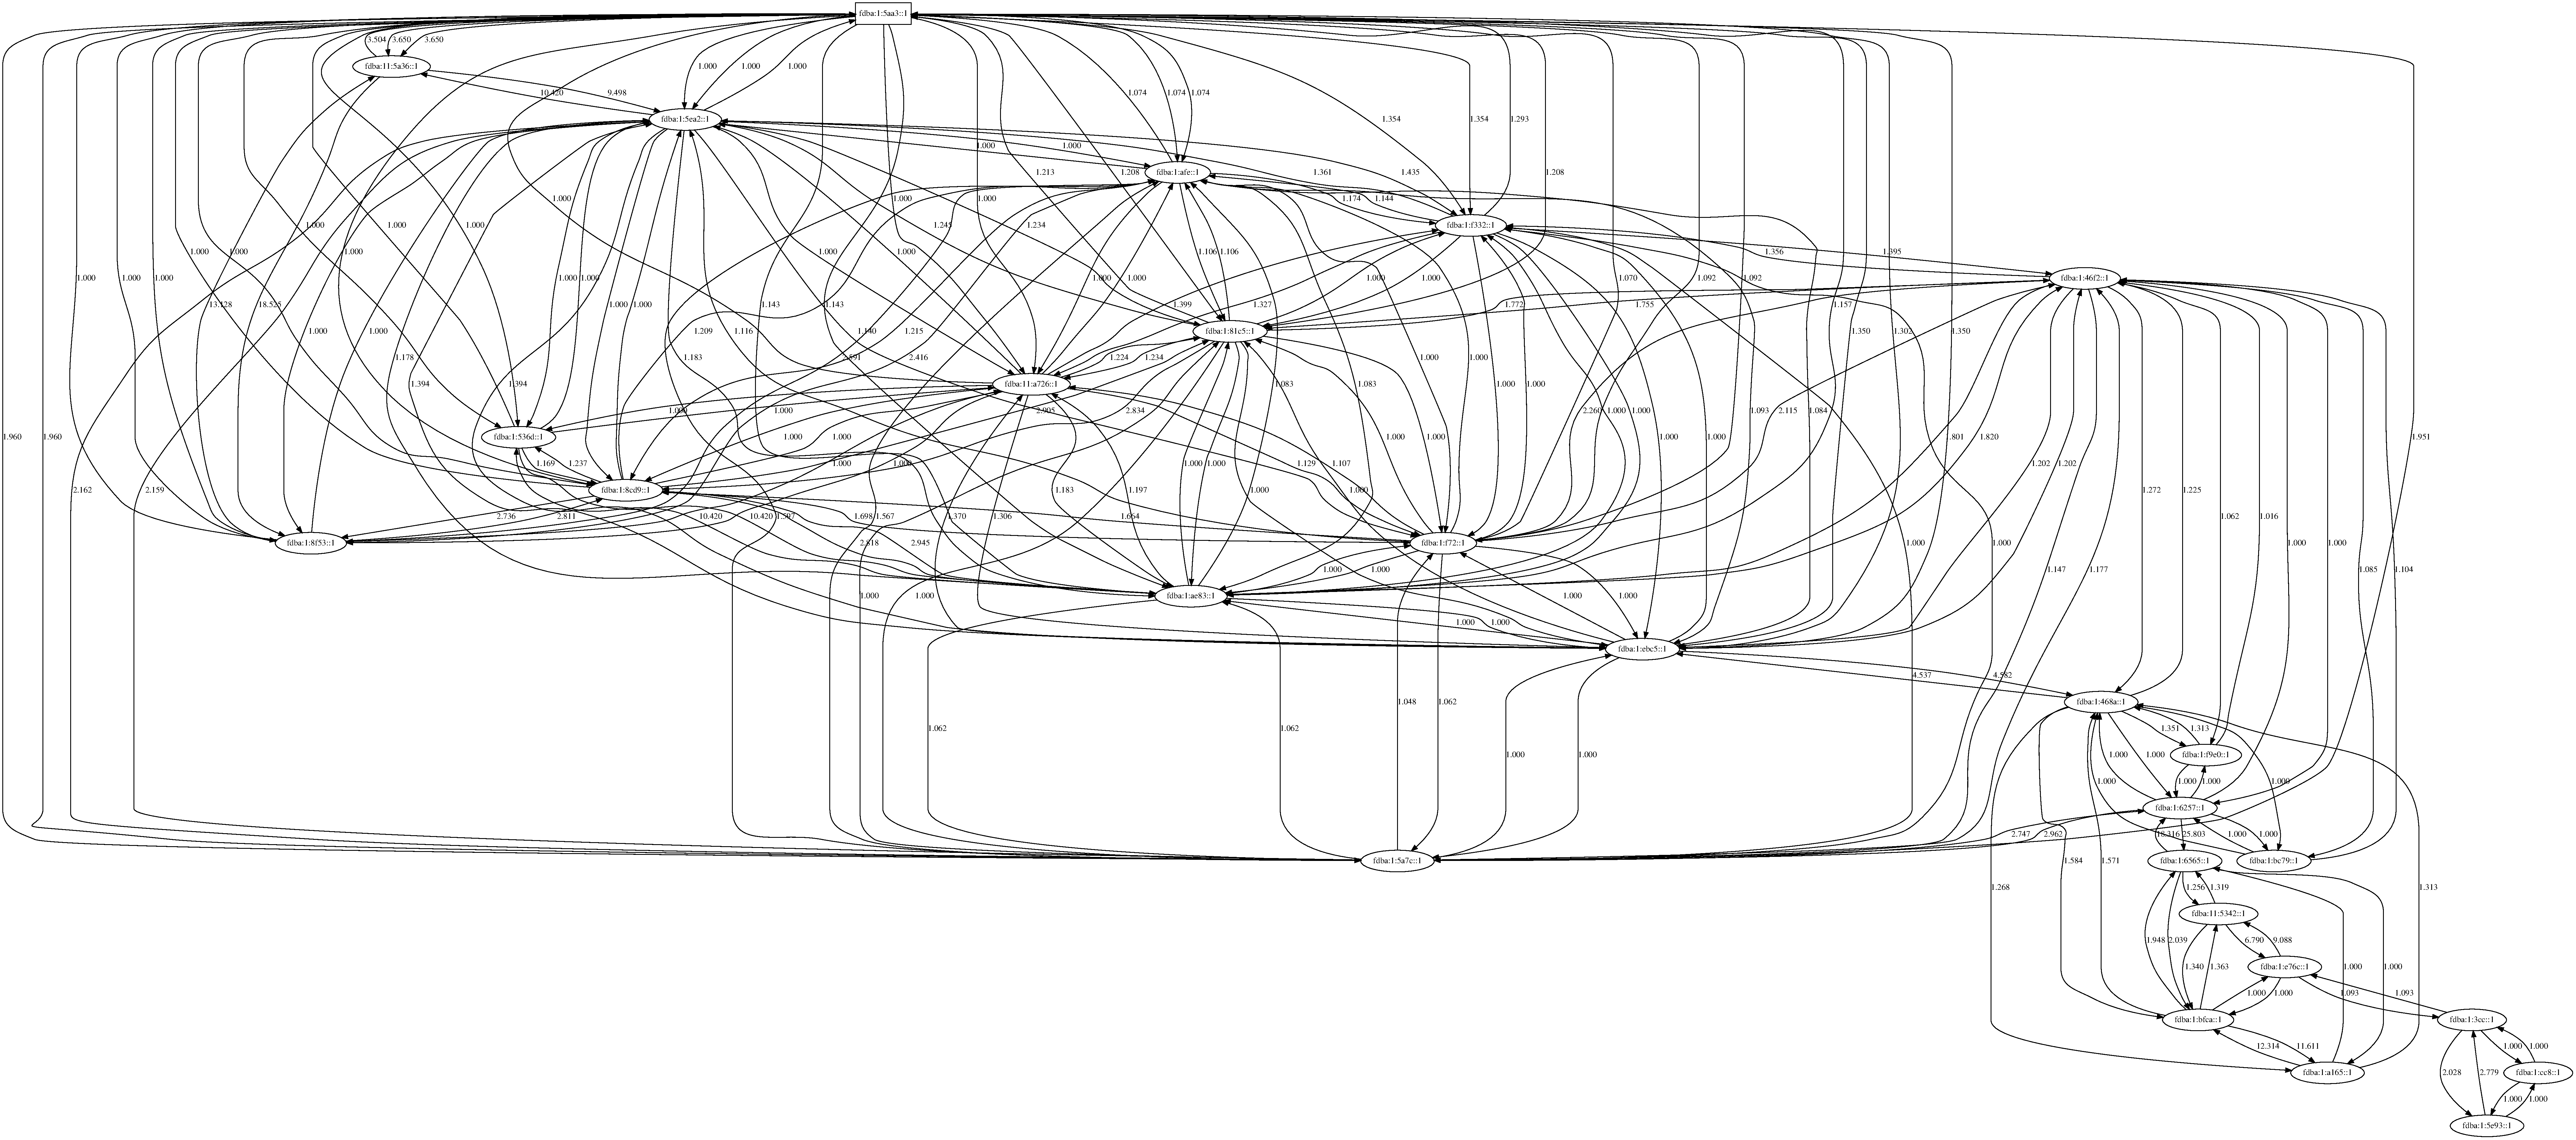
\includegraphics[width=1.4\textwidth, angle=90]{figures/topo0.pdf}
\caption{OLSR topology snapshot}
\label{fig:olsr-topo}
\end{figure}

%\begin{figure}[h]
%\centering
%\def\svgwidth{\columnwidth}
%\includesvg{topo0}
%\end{figure}

\clearpage

%%%%%%%%%%%%%%%%%%%%%%%%%%%%%%%%%%%%%%%%%%%%%%%%%%%%%%%%%%%%%%%%%%%%%%%%%%%%%%%%
%%%%%%%%%%%%%%%%%%%%%%%%%%%%%%%%%%%%%%%%%%%%%%%%%%%%%%%%%%%%%%%%%%%%%%%%%%%%%%%%
%%%%%%%%%%%%%%%%%%%%%%%%%%%%%%%%%%%%%%%%%%%%%%%%%%%%%%%%%%%%%%%%%%%%%%%%%%%%%%%%
\section{Ping Measurements (hops, rtt, loss)}
\label{sec:ping-measurements}

%%%%%%%%%%%%%%%%%%%%%%%%%%%%%%%%%%%%%%%%%%%%%%%%%%%%%%%%%%%%%%%%%%%%%%%%%%%%%%%%
\subsection{Assumptions}

Like always, when post-processing the measurement data obtained during
an event several weeks ago one notices that some particular
information was not logged and may question the validity of the
analysis. 

The main problem identified from the WBMv6 measurement is the
phenomenon that the ping program, although configured to send a fixed
number of icmp probes at a given interval, does in-fact not complete
the task in the expected time.  For example one would expect that 100
pings send at an interval of 100ms would finish after 10s. But usually
much longer periods have been observed. One reason for this effect is
given by link-layer address resolution. It clearly seems that the time
needed for resolving the link-layer address for forwarding a packet to
the first hop (from layer 3 perspective) towards the destination is
not counted for the overall round trip time. Instead, the whole
process is delayed respectively. This claim can be confirmed with the
experiment in Section \ref{arp-resolution}.


The described behavior affects the measurements in the following ways:

For the stationary scenarios as analyzed in Sections \ref{stationary},
ping has been configured to measure 1000 round-trip times at an
interval of 100 ms. Some experiments indeed completed this task in the
foreseen time of 10000ms (eg groups 17,18,19, see GRP and TIME column
of Table \ref{tab:} and Figures \ref{tab:}).  However, in other cases
it happened that pings send using one or several protocols took much
longer (eg groups 5, see GRP and TIME column of Table \ref{tab:} and
Figures \ref{tab:}) where although all protocols showed zero packet
loss, bmx6 took 30\% more time to send the 1000 pings than babel. 

I believe that the corresponding routing protocol can be accounted
for the long delays and should be penalized as its the routing
protocol's job to find a good next hops (with low arp-resolution
delays). Also, if the ping command would have continued to count time
during the resolution delays, all pings send within this period would
got lost or at least show a significantly greater RTT. Further, as
these delays are only ignored on the first hop (from layer 3
perspective) while arp-delays occurring beyond the first hop are indeed
counted by the reported RTT, a layer-2 routing protocol would gain
unfair benefits if ignoring these delays.


Therefore, simply comparing the successful ping replies would not be
fair as the objective was to send them in the given time.  To
compensate this, the same fraction of icmp probes was considered as
lost for the analysis as the total measurement time exceeded the
foreseen time. As an example, if 8 pings send at an interval of 100ms
took twice the expected time to complete (1600ms instead of 800ms)
then 50\% of the observed icmp probes are considered as lost for the
analysis.  So in case 1,3,5,8 (of 1-8) were received then 50\% (using
the greatest aware sequence numbers: 5,6,7,8) are discarded, resulting
in a reduced total success rate of only 25\% (instead of 50\%).

Applying this kind of penalty was possible for the stationary (random)
measurements as all traces included the finishing summary which includes
the total time used for the measurement.
For the mobile scenarios, a different assumption was made because the ping
traces did not include this summary. Probably because ping was killed manually
when the test-run was finished. Therefore it was assumed that all test-runs
took roughly the same time (the persons moving the mobile node did not move
significantly faster when testing a particular protocol) and the maximum 
received sequence number of each experiment was considered unless this 
number differed significantly from the maximum received sequence number 
observed in all experiments.

Further, all Figures shown in this Section include only measurements where
each participating protocol succeeded with a minimum amount of probes.

In contrast, the Appendix also includes measurements (groups) where only
a subset of protocols succeeded.



\subsubsection{Understanding uncounted ping delays}
\label{arp-resolution}
How arp/lladdr resolution affects ping interval

This section shows how failing (or long lasting) arp/lladdr resolution
causes ping to emit icmp probes at a lower interval than specified,
This can result in less total send pings during a given time.
Therefore I set up a virtual network environment with a high
broadcast/multicast packet loss but zero unicast packet loss.
The following three experiments prove this strange ping behavior.
IMHO, these ``non-send'' pings should be accounted as lost pings when
comparing routing-protocols ping performance with each other.



\begin{verbatim}
1. Experiment: arp/lladr is resolved,
    As expected 100 pings at 0.1s interval take ~10 seconds!

root@mlc1001:~# ip neigh
fe80::a2cd:efff:fe10:201 dev eth1 lladdr a0:cd:ef:10:02:01 router REACHABLE

root@mlc1001:~# ping6 -q -c100 -i0.1 fd66:66:66:2c:a2cd:efff:fe10:201 &
PING fd66:66:66:2c:a2cd:efff:fe10:201(fd66:66:66:2c:a2cd:efff:fe10:201) 56 data bytes
--- fd66:66:66:2c:a2cd:efff:fe10:201 ping statistics ---
100 packets transmitted, 100 received, 0% packet loss, time 10068ms
rtt min/avg/max/mdev = 800.119/800.231/800.331/0.717 ms, pipe 8



2. Experiment: arp/lladr still resolved but flushed three times during ping!
    Surprisingly 100 pings ``at 0.1s interval'' take ~15 seconds!

root@mlc1001:~# ping6 -q -c100 -i0.1 fd66:66:66:2c:a2cd:efff:fe10:201 &
PING fd66:66:66:2c:a2cd:efff:fe10:201(fd66:66:66:2c:a2cd:efff:fe10:201) 56 data bytes
root@mlc1001:~# ip neigh flush dev eth1
root@mlc1001:~# ip neigh flush dev eth1
root@mlc1001:~# ip neigh flush dev eth1
--- fd66:66:66:2c:a2cd:efff:fe10:201 ping statistics ---
100 packets transmitted, 86 received, +14 errors, 14% packet loss, time 15878ms
rtt min/avg/max/mdev = 800.133/891.637/2203.781/299.134 ms, pipe 14



3. Experiment: arp/lladr flushed three times during ping and SIGINT send to ping after 11 seconds!
    Only 69 pings ``at 0.1s interval'' send in ~10 seconds!

root@mlc1001:~# ping6 -q -c100 -i0.1 fd66:66:66:2c:a2cd:efff:fe10:201 & (sleep 11; killall -2 ping6) &
PING fd66:66:66:2c:a2cd:efff:fe10:201(fd66:66:66:2c:a2cd:efff:fe10:201) 56 data bytes
root@mlc1001:~# ip neigh flush dev eth1
root@mlc1001:~# ip neigh flush dev eth1
root@mlc1001:~# ip neigh flush dev eth1
--- fd66:66:66:2c:a2cd:efff:fe10:201 ping statistics ---
69 packets transmitted, 57 received, +6 errors, 17% packet loss, time 10919ms
rtt min/avg/max/mdev = 800.144/919.743/2202.364/353.556 ms, pipe 14
\end{verbatim}






%%%%%%%%%%%%%%%%%%%%%%%%%%%%%%%%%%%%%%%%%%%%%%%%%%%%%%%%%%%%%%%%%%%%%%%%%%%%%%%%
%\immediate\write18{ ../eval.R --data=../tmp.data --stat=../tmp.stat --imgdir=../img --texdir=inputs/ }

%%%%%%%%%%%%%%%%%%%%%%%%%%%%%%%%%%%%%%%%%%%%%%%%%%%%%%%%%%%%%%%%%%%%%%%%%%%%%%%%
\subsection{Stationary Scenarios}

\clearpage
\makeFigure{sArtt}{Random node test 1}{0.69} \makeFigure{sArvh}{Random
  node test 1}{0.69}

\clearpage

\makeFigure{sBrtt}{Random node test 2}{0.69}
\makeFigure{sBrvh}{Random node test 2}{0.69}


\clearpage

%%%%%%%%%%%%%%%%%%%%%%%%%%%%%%%%%%%%%%%%%%%%%%%%%%%%%%%%%%%%%%%%%%%%%%%%%%%%%%%%
\subsection{Mobile Scenarios}


%\makeFigure{sArtt}{RTT ECDF of mobile and running node tests (groups 1-3)}{0.7}
%\makeFigure{sArvh}{RTT vs hops of Mobile and running node tests (groups 1-3)}{0.7}


\makeCCTabl{tbl:m0}{Mobile test 0 (group 1)} {%
      \makeTCCGraphic{m0}
}

\makeCCTabl{tbl:m1}{Mobile node test 1 (group 2)} {%
      \makeTCCGraphic{m1}
}

\makeCCTabl{tbl:m0-m2}{Running node test 2 (group 3)} {%
      \makeTCCGraphic{m2}
}



%\begin{figure}
% \centering
% \includegraphics[width=1\textwidth]{../img/out.pdf}
% \caption{Research guidelines}
% \label{fig:guidelines}
%\end{figure}


%%%%%%%%%%%%%%%%%%%%%%%%%%%%%%%%%%%%%%%%%%%%%%%%%%%%%%%%%%%%%%%%%%%%%%%%%%%%%%%%
%%%%%%%%%%%%%%%%%%%%%%%%%%%%%%%%%%%%%%%%%%%%%%%%%%%%%%%%%%%%%%%%%%%%%%%%%%%%%%%%
%%%%%%%%%%%%%%%%%%%%%%%%%%%%%%%%%%%%%%%%%%%%%%%%%%%%%%%%%%%%%%%%%%%%%%%%%%%%%%%%
\section{TCP Throughput Measurements}
\label{sec:tp-measurements}




\section{Recommendations for next battlemesh}

\begin{itemize}

\item Terminate running pings with SIGINT (eg killall -SIGINT ping6) instead of SIGKILL (eg killall ping6). This will cause ping to still print the ping statistics

\item Run top so that it makes a second measurement over a reasonable time (eg 5 seconds). Otherwise the cpu measurements are useless as they only present the cpu usage over a fraction of a second. This can be achieved with arguments "top -b -n 2 -d 2 "

\item Traceroute and mrt often show  high packet for intermediate nodes. This is due to a kind of denial-of-service mechanism enabled by default in Linux kernel. WIth this mechanism the kernel simply discards frequent icmp responses (eg due to exceeded TTL values). This behavior can be disabled by lowering the default net.ipv6.icmp.ratelimit=1000 setting, eg via: sysctl -w net.ipv6.icmp.ratelimit=10

\item Most important: Measure protocol traffic overhead in parallel
\end{itemize}


%%%%%%%%%%%%%%%%%%%%%%%%%%%%%%%%%%%%%%%%%%%%%%%%%%%%%%%%%%%%%%%%%%%%%%%%%%%%%%%%
%%%%%%%%%%%%%%%%%%%%%%%%%%%%%%%%%%%%%%%%%%%%%%%%%%%%%%%%%%%%%%%%%%%%%%%%%%%%%%%%
%%%%%%%%%%%%%%%%%%%%%%%%%%%%%%%%%%%%%%%%%%%%%%%%%%%%%%%%%%%%%%%%%%%%%%%%%%%%%%%%
\section{Appendix}

\subsection{Ping Results Table}

The folloing verbatim table lists statistics per experiment (EXP) and group (GRP) as calculated by the lua-based
evaluation script based on the raw ping-measurements data and outputted to the file ping.stat.
Event based results are given for each received icmp response in ping.data.

% redefine \VerbatimInput
\RecustomVerbatimCommand{\VerbatimInput}{VerbatimInput}%
{fontsize=\tiny,
 %
 frame=lines,  % top and bottom rule only
 framesep=2em, % separation between frame and text
% rulecolor=\color{Gray},
 %
 label=\fbox{ping.stat},
 labelposition=topline,
 %
 commandchars=\|\(\), % escape character and argument delimiters for
                      % commands within the verbatim
 commentchar=*        % comment character
}

\VerbatimInput{../ping.stat}

\subsection{Individual Random-node Test Measurements}

\makeCCCTabl{tbl:s4-s6}{Individual Random node tests (groups 4-6)} {%
      \makeCCCGraphic{s4}
      \makeCCCGraphic{s5}
      \makeCCCGraphic{s6}
      \makeCCCGraphic{s7}
}

\makeCCCTabl{tbl:s4-s6}{Individual Random node tests (groups 8-11)} {%
      \makeCCCGraphic{s8}
      \makeCCCGraphic{s9}
      \makeCCCGraphic{s10}
      \makeCCCGraphic{s11}
}

\makeCCCTabl{tbl:s4-s6}{Individual Random node tests (groups 12-15)} {%
      \makeCCCGraphic{s12}
      \makeCCCGraphic{s13}
      \makeCCCGraphic{s14}
      \makeCCCGraphic{s15}
}

\makeCCCTabl{tbl:s4-s6}{Individual Random node tests (groups 16-19)} {%
      \makeCCCGraphic{s16}
      \makeCCCGraphic{s17}
      \makeCCCGraphic{s18}
      \makeCCCGraphic{s19}
}

\makeCCCTabl{tbl:s4-s6}{Individual Random node tests (groups 20-23)} {%
      \makeCCCGraphic{s20}
      \makeCCCGraphic{s21}
      \makeCCCGraphic{s22}
      \makeCCCGraphic{s23}
}

\makeCCCTabl{tbl:s4-s6}{Individual Random node tests (groups 24-27)} {%
      \makeCCCGraphic{s24}
      \makeCCCGraphic{s25}
      \makeCCCGraphic{s26}
      \makeCCCGraphic{s27}
}

\makeCCCTabl{tbl:s4-s6}{Individual Random node tests (groups 28-31)} {%
      \makeCCCGraphic{s28}
      \makeCCCGraphic{s29}
      \makeCCCGraphic{s30}
      \makeCCCGraphic{s31}
}

\makeCCCTabl{tbl:s4-s6}{Individual Random node tests (groups 32-35)} {%
      \makeCCCGraphic{s32}
      \makeCCCGraphic{s33}
      \makeCCCGraphic{s34}
      \makeCCCGraphic{s35}
}

\makeCCCTabl{tbl:s4-s6}{Individual Random node tests (groups 36-39)} {%
      \makeCCCGraphic{s36}
      \makeCCCGraphic{s37}
      \makeCCCGraphic{s38}
      \makeCCCGraphic{s39}
}

\makeCCCTabl{tbl:s4-s6}{Individual Random node tests (groups 40-43)} {%
      \makeCCCGraphic{s40}
      \makeCCCGraphic{s41}
      \makeCCCGraphic{s42}
      \makeCCCGraphic{s43}
}

\makeCCCTabl{tbl:s4-s6}{Individual Random node tests (groups 44-47)} {%
      \makeCCCGraphic{s44}
      \makeCCCGraphic{s45}
      \makeCCCGraphic{s46}
      \makeCCCGraphic{s47}
}

\makeCCCTabl{tbl:s4-s6}{Individual Random node tests (groups 48-50)} {%
      \makeCCCGraphic{s48}
      \makeCCCGraphic{s49}
      \makeCCCGraphic{s50}
}


%%%%%%%%%%%%%%%%%%%%%%%%%%%%%%%%%%%%%%%%%%%%%%%%%%%%%%%%%%%%%%%%%%%%%%%%%%%%%%%%
%%%%%%%%%%%%%%%%%%%%%%%%%%%%%%%%%%%%%%%%%%%%%%%%%%%%%%%%%%%%%%%%%%%%%%%%%%%%%%%%
%\section*{Acknowledgements}
%
%This work is supported by ...


%%%%%%%%%%%%%%%%%%%%%%%%%%%%%%%%%%%%%%%%%%%%%%%%%%%%%%%%%%%%%%%%%%%%%%%%%%%%%%%%
%%%%%%%%%%%%%%%%%%%%%%%%%%%%%%%%%%%%%%%%%%%%%%%%%%%%%%%%%%%%%%%%%%%%%%%%%%%%%%%%

\backmatter

\bibliographystyle{ieeetr}
%\bibliography{biblio-data}

\end{document} 
